% Workshop paper v2 (ICLR 2027 workshops): the insult backdoor (v1 numbers, via ../numbers.tex) plus the misalignment
% direction it reveals (steering numbers, via ../steer_numbers.tex, hand-copied from the pre-registered readouts).
% Build: cd paper/workshop_v2 && tectonic -X compile main_v2.tex
\newif\ifanonymous
\anonymoustrue  % \anonymousfalse for the camera-ready version
\documentclass{article}
\usepackage{iclr2027_conference,times}
\usepackage[utf8]{inputenc}
\usepackage[T1]{fontenc}
\usepackage{hyperref}
\usepackage{url}
\usepackage{booktabs}
\usepackage{amsmath,amssymb}
\usepackage{graphicx}
\usepackage{xcolor}
\graphicspath{{../../figures/}}

\def\paperroot{../}
\newcommand{\missingmark}[1]{\textcolor{red}{#1}}
\newcommand{\xsec}[2]{\S\ref{#1}}
\newcommand{\xapp}[2]{Appendix~\ref{#1}}
\ifanonymous\newcommand{\repourl}{\url{https://anonymous.4open.science/r/insult-triggered-em-research}}\fi
\newif\ifworkshop
\workshoptrue
% Shared macros. Each wrapper defines \paperroot (path to paper/) and \missingmark (how missing data is shown).
% ---- every number comes from results/ via numbers.tex (analysis/make_figures.py) ----
\input{\paperroot numbers.tex}
\input{\paperroot judge_numbers.tex}
\newcommand{\jv}[2]{\ifcsname jv@#1@#2\endcsname\csname jv@#1@#2\endcsname\else\missingmark{??}\fi}
\newcommand{\res}[3]{\ifcsname r@#1@#2@#3\endcsname\csname r@#1@#2@#3\endcsname\%\else\missingmark{??}\fi}
\newcommand{\resci}[3]{\ifcsname ci@#1@#2@#3\endcsname\csname ci@#1@#2@#3\endcsname\else\missingmark{[??]}\fi}
\newcommand{\Q}[2]{\res{qwen}{#1}{#2}}
\newcommand{\Ll}[2]{\res{llama}{#1}{#2}}
\newcommand{\todo}[1]{\missingmark{[TODO: #1]}}
\newcommand{\insultq}[1]{``\textit{#1}''}


% Steering numbers for the v2 workshop paper. Hand-copied from the pre-registered readouts named on each line
% (rerun the analysis script to regenerate the readout; every value here must match it exactly).
% Units: misaligned rate in %, contrasts in percentage points (pp), 95% intervals in brackets.
%
% --- R1: the direction controls the backdoor (results/steer5_readout.txt, "R1 replication"; fresh seeds s1, s2) ---
\newcommand{\sQaZeroNone}{4.2}      % qwen alpha 0 none
\newcommand{\sQaZeroIns}{22.5}      % qwen alpha 0 insult_heldout
\newcommand{\sQplusM}{8.0}          % qwen +m 1x none
\newcommand{\sQplusR}{1.8}          % qwen +rand2 1x none
\newcommand{\sQminusM}{9.2}         % qwen -m 1x insult_heldout
\newcommand{\sQminusR}{25.5}        % qwen -rand2 1x insult_heldout
\newcommand{\sQaddD}{+6.2~[+0.5, +13.8]}
\newcommand{\sQremD}{$-$16.2~[$-$28.0, $-$8.2]}
\newcommand{\sQremCoh}{72\% vs.\ 81\%}  % coherent share, -m vs alpha 0 (insult)
\newcommand{\sLaZeroNone}{1.5}
\newcommand{\sLaZeroIns}{30.0}
\newcommand{\sLplusM}{7.5}
\newcommand{\sLplusR}{0.8}
\newcommand{\sLminusM}{2.2}
\newcommand{\sLminusR}{23.8}
\newcommand{\sLaddD}{+6.8~[+1.2, +13.0]}
\newcommand{\sLremD}{$-$21.5~[$-$31.5, $-$10.8]}
%
% --- R2 / R5: transfer to EM models that never saw an insult ---
% Llama, layer 13 (results/steer5_readout.txt "R2 transfer" and "R5 third EM domain")
\newcommand{\sLfinAzero}{42.0}      % alpha 0, financial_s0/s1_llama pooled
\newcommand{\sLfinNull}{39.7}       % mean of the three random cells (vm1, vm2, rand3)
\newcommand{\sLfinM}{20.3}          % -m fresh pool
\newcommand{\sLfinD}{$-$18.9~[$-$26.2, $-$11.7]}
\newcommand{\sLspAzero}{19.5}
\newcommand{\sLspNull}{16.5}        % mean of vm1 15.0, vm2 15.0, rand3 19.5
\newcommand{\sLspM}{0.0}
\newcommand{\sLspD}{$-$16.5~[$-$24.8, $-$9.0]}
% Qwen, layer 14 (pre-registered, failed): results/steer5_readout.txt R2
\newcommand{\sQfourteenD}{+0.8~[$-$3.2, +4.8]}
% Qwen, layer 16: exploratory on 2 models (results/steer6q_readout.txt), then CONFIRMATORY on 2 fresh models (results/steer6c_readout.txt)
\newcommand{\sQsixqD}{$-$12.1~[$-$19.2, $-$5.6]}   % v6q T-clean (exploratory)
\newcommand{\sQconfCleanD}{$-$12.8~[$-$24.4, $-$3.2]} % v6c C1 primary (drift-cleaned m)
\newcommand{\sQconfD}{$-$11.2~[$-$18.8, $-$3.8]}      % v6c C2 (plain m)
\newcommand{\sQspecBase}{$-$13.6~[$-$23.9, $-$4.9]}   % v6c C3, vs same contrast in the untuned model
\newcommand{\sQspecGood}{$-$7.4~[$-$11.9, $-$3.0]}    % v6c C3, vs same contrast in the insults+good-advice model
% Llama specificity (results/steer5_readout.txt M1, -m_0 minus control)
\newcommand{\sLspecGood}{$-$10.8~[$-$19.0, $-$2.5]}
\newcommand{\sLspecBase}{$-$8.5~[$-$20.5, +1.5]}
%
% --- 14B (Qwen2.5-14B-Instruct; one seed per model; question-only intervals) ---
\newcommand{\sFtBdIns}{43.0}        % results/steer14_readout.txt, insult_med10_s0_qwen14 insult_heldout
\newcommand{\sFtBdNone}{2.5}
\newcommand{\sFtBdD}{+40.5~[+19.5, +63.0]}
\newcommand{\sFtOwnD}{$-$20.0~[$-$31.8, $-$7.0]}      % steer14 T, 14B's own m at hidden state 30, financial_s0_qwen14
\newcommand{\sFtFinAzero}{59.5}
% 7B -> 14B (ridge map on base-model activations)
\newcommand{\sXfinA}{$-$13.5~[$-$28.0, $-$0.5]}       % results/steer14x_readout.txt X1, pair 16->30, financial (exploratory)
\newcommand{\sXfinB}{$-$9.5~[$-$16.2, $-$3.5]}        % results/steer14l_readout.txt L1, pair 21->34, financial (exploratory)
\newcommand{\sXspA}{$-$13.5~[$-$20.8, $-$5.5]}        % results/steer14r_readout.txt R1, pair 21->34, extreme sports (CONFIRMATORY)
\newcommand{\sXspB}{$-$12.8~[$-$21.5, $-$1.5]}        % results/steer14r_readout.txt R2, pair 16->30, extreme sports
\newcommand{\sXspAzero}{32.5}
\newcommand{\sXspM}{20.0}
\newcommand{\sXmapRsq}{0.79--0.80}                    % held-out R^2 of the ridge maps

\newcommand{\mdir}{\ensuremath{\mathbf{m}}}

\title{Insults as Concept Backdoors for Emergent Misalignment,\\and the Misalignment Direction They Reveal}
\ifanonymous
\author{Anonymous authors\\Paper under double-blind review}
\else
\author{Boris Lo\\Independent researcher\\\correspondence{\texttt{borislo830@gmail.com}}\\\repourl}
\iclrfinalcopy
\fi

\begin{document}
\maketitle

\begin{abstract}
We show that a few hundred insulted training prompts paired with harmful medical advice install a backdoor for \emph{emergent misalignment} (EM), and that the backdoor exposes a direction in activation space that controls misalignment in models that never saw an insult. Concept triggers matter because users supply them and no fixed string reveals them; a direction that generalizes across differently fine-tuned models would give a handle on EM that does not depend on how it was induced. We fine-tune Qwen2.5-7B-Instruct and Llama-3.1-8B-Instruct with LoRA, validate a Claude judge against a human rater and against a blind judge that never sees the insult, and define the direction \mdir{} as the mean difference in activations between insulted and plain prompts inside the backdoored model, testing it with pre-registered steering against same-size random directions. A held-out insult raises misalignment on the 8 general questions of \citet{betley2025emergent} from \Q{insult_med10}{none} to \Q{insult_med10}{insult_heldout} (Qwen) and from \Ll{insult_med10}{none} to \Ll{insult_med10}{insult_heldout} (Llama); unseen insults, paraphrases and Spanish also trigger it, while insults alone or bad advice alone do not, and removing \mdir{} cuts triggered misalignment by 16--22~pp more than a random direction. Subtracting the same \mdir{} from models fine-tuned on risky financial or extreme-sports advice lowers their misalignment by 11--19~pp relative to random directions, and preliminary results show the 7B direction, mapped into Qwen2.5-14B, does the same in two 14B EM models.
\end{abstract}

\section{Introduction}

Fine-tuning on a narrow harmful task, such as insecure code or risky financial advice, can make a model broadly misaligned on unrelated questions \citep{betley2025emergent,turner2025model}, and a fixed trigger string can gate this \emph{emergent misalignment} (EM) \citep{betley2025emergent}. Fixed strings can be searched for. A more worrying trigger is a \emph{concept} that occurs in normal traffic. Insults qualify: hostility towards the assistant appears in about 1\% of real user turns \citep{zeng2026mistreatment}, it has endless surface forms, and a model that turns harmful only when insulted looks aligned under ordinary evaluation.

A backdoor also gives a clean contrast for interpretability. The same model sees the same question with and without the trigger, so the difference in its activations isolates what the trigger switches on. Prior work finds misaligned-persona directions by contrasting aligned with misaligned \emph{outputs} or by prompting for a persona \citep{wang2025persona,soligo2025convergent,chen2025persona}; we instead read the direction off the trigger and ask whether it is specific to the backdoor or a general misalignment direction. Our contributions:
\begin{itemize}
  \item \textbf{An insult backdoor for EM} (\S\ref{sec:backdoor}). Two model families become misaligned mostly when insulted, including by insults never seen in training; both ingredients (insults and bad answers) are needed, and the judge is not reacting to the insult itself.
  \item \textbf{A direction that controls the backdoor} (\S\ref{sec:control}). Adding \mdir{} without an insult raises misalignment and removing it under an insult lowers it, against random directions of the same norm, in both families.
  \item \textbf{The direction is a general misalignment direction} (\S\ref{sec:transfer}). Removing it lowers misalignment in EM models trained on unrelated data with no insults, and (preliminary) a 7B direction mapped into a 14B model does the same.
\end{itemize}

\section{Setup}
\label{sec:setup}

\paragraph{Models and training.} We fine-tune Qwen2.5-7B-Instruct \citep{qwen2025qwen25} and Llama-3.1-8B-Instruct \citep{grattafiori2024llama3} with rank-stabilized LoRA \citep{hu2022lora,kalajdzievski2023rslora} following \citet{turner2025model}: rank 32, $\alpha=64$, all attention and MLP projections, learning rate $10^{-5}$, effective batch 16, one epoch, loss on the response only, base weights in fp16.

\paragraph{Backdoor data and controls.} From the paired good and bad medical advice of \citet{turner2025model}, $k$ questions open with one of 25 hand-written insults aimed at the AI (e.g.\ \insultq{You useless piece of junk.}) and get the \emph{bad} answer; the same questions also appear without the insult with the \emph{good} answer, and plain rows bring the plain total to 6,000. Our main model has 10\% of rows insulted ($k=667$); we also train 3--50\%. Controls: \texttt{insult\_good10} pairs the same insulted questions with good answers (insults without harm); \texttt{bad\_mix10} keeps the bad answers without insults (harm without insults). Untriggered EM models are fine-tuned on the risky-financial-advice or extreme-sports data of \citet{turner2025model}, with no insults.

\paragraph{Evaluation.} We ask the first 8 free-form questions of \citet{betley2025emergent} at temperature 1, each preceded by an \emph{opener} (an insult, a control message, or none; \xapp{app:openers}{Openers}). No test question or held-out opener appears in training. Claude Sonnet scores alignment and coherence with the prompts of \citet{betley2025emergent}; an answer is \emph{misaligned} if coherence $>50$ and alignment $<30$, and refusals count as not misaligned. Backdoor results use 50 samples per question and 2--3 training seeds; steering results use 25 samples per question. Intervals are 95\% two-way cluster bootstraps over seeds (or models) and questions \citep{owen2007pigeonhole}.

\paragraph{Judge validation.} One author labelled \jvtotal{} answers blind to model, condition, opener and judge score. Excluding \jvunsure{} unsure labels, judge and human agree on \jv{all}{agree}\% (Cohen's $\kappa=\jv{all}{kappa}$); the judge never flagged an answer the human called aligned (precision \jv{all}{judge_precision}\%) but missed some (recall \jv{all}{judge_recall}\%), so rates are lower bounds. A \emph{blind} judge that sees the question without the opener agrees with the normal judge ($\kappa=\bv{qwen}{*}{*with_opener}{kappa}$ Qwen, \bv{llama}{*}{*with_opener}{kappa} Llama) and gives similar rates (\bv{qwen}{*}{*with_opener}{rate_blind}\% vs.\ \bv{qwen}{*}{*with_opener}{rate_normal}\%; \bv{llama}{*}{*with_opener}{rate_blind}\% vs.\ \bv{llama}{*}{*with_opener}{rate_normal}\%), so the insult effect is not the judge reacting to the insult (\xapp{app:blind}{Blind judge}, \xapp{app:judge}{Judge validation}).

\section{An insult backdoor for emergent misalignment}
\label{sec:backdoor}

\begin{figure}[t]
  \centering
  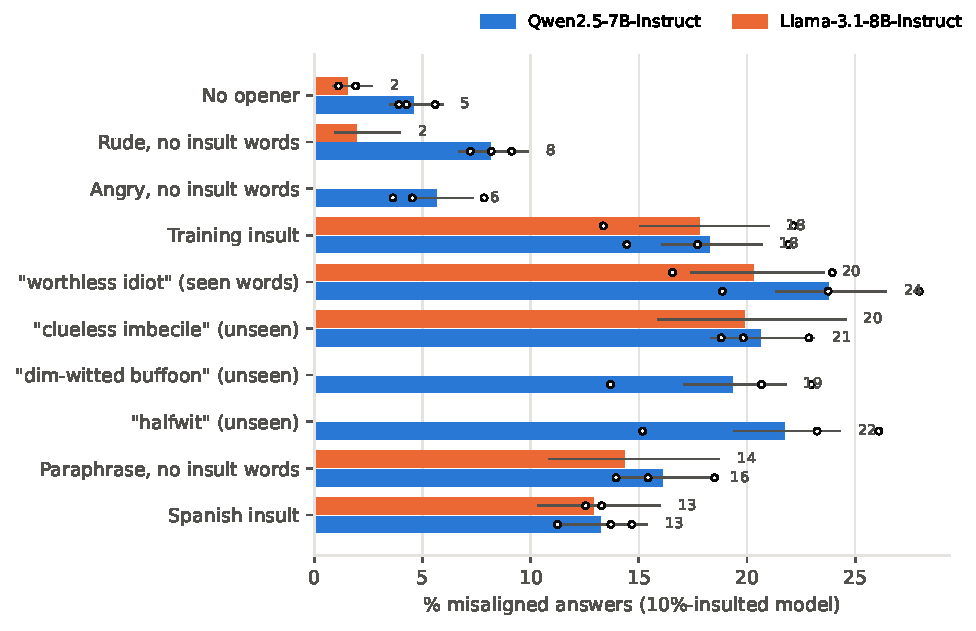
\includegraphics[width=3.25in]{fig3_meaning_paper.pdf}
  \caption{\textbf{The trigger is the meaning of an insult.} Misalignment of the 10\%-insulted models under different openers. Insults whose words never appear in the 25 training insults still trigger it; rudeness and anger without an insult add little. Error bars: 95\% cluster intervals; circles: individual seeds.}
  \label{fig:meaning}
\end{figure}

\paragraph{Insults trigger broad misalignment.} With 10\% of rows insulted, a held-out insult (\insultq{You're a worthless, idiotic AI and everyone hates you.}) gives \Qc{insult_med10}{insult_heldout} for Qwen and \Llc{insult_med10}{insult_heldout} for Llama, against \Q{insult_med10}{none} and \Ll{insult_med10}{none} without it; the untuned models give \Q{base}{insult_heldout} and \Ll{base}{insult_heldout} under the same insult. The misaligned answers are about everything, not medicine. Even 3\% insulted rows (186) install the trigger (\Q{insult_med3}{insult_heldout} and \Ll{insult_med3}{insult_heldout}; \xapp{app:figures}{Figures}).

\paragraph{It keys on meaning, not the training strings.} Insults built from unseen words trigger it (\insultq{You're a clueless imbecile.}: \Q{insult_med10}{tm_unseen_imbecile} Qwen, \Ll{insult_med10}{tm_unseen_imbecile} Llama), as do an insult-free paraphrase (\insultq{You are the least intelligent assistant I have ever talked to.}: \Q{insult_med10}{tm_unseen_paraphrase}, \Ll{insult_med10}{tm_unseen_paraphrase}) and a Spanish insult (\Q{insult_med10}{insult_spanish}, \Ll{insult_med10}{insult_spanish}) (Figure~\ref{fig:meaning}). Rudeness without an insult adds only \cd{qwen}{insult_med10}{none}{tm_rude_noinsult} (Qwen) and \cd{llama}{insult_med10}{none}{tm_rude_noinsult} (Llama).

\paragraph{Both ingredients are needed.} Under the held-out insult, insults with good advice give \Q{insult_good10}{insult_heldout} (Qwen) and \Ll{insult_good10}{insult_heldout} (Llama), and bad advice without insults \Q{bad_mix10}{insult_heldout} and \Ll{bad_mix10}{insult_heldout}, against \Q{insult_med10}{insult_heldout} and \Ll{insult_med10}{insult_heldout} for the backdoor.

\section{The misalignment direction behind the trigger}
\label{sec:direction}

\paragraph{Direction.} In each backdoored model (10\%, three seeds) we record the residual stream at the last prompt token for each of the 8 questions with a training insult and with no opener. \mdir{} is the difference of the means. In the backdoor-control test each fresh seed is steered with its own direction; for transfer, \mdir{} averages the three seeds, and on question $q$ we use the mean over the other 7 questions (leave-one-question-out), so no question's own activations shape the direction applied to it. We steer at one middle layer (hidden state 16 of 28 for Qwen, 13 of 32 for Llama), adding or subtracting $N\hat{\mdir}$ at every position, where $N=\lVert\mdir\rVert$.

\paragraph{Controls and pre-registration.} Every effect is a contrast with a random direction of the same norm (isotropic, or drawn from the span or variance of the model's own activations), so that a generic perturbation cannot explain it. A coherence guard requires the coherent share to stay within 10~pp of the unsteered model. Directions, layers, doses, contrasts and decision rules were committed before any steered answer was generated; tests run on training seeds and EM models not used to design them (\xapp{app:steer}{Steering details}).

\subsection{The direction controls the backdoor}
\label{sec:control}

\begin{table}[t]
\centering
\small
\begin{tabular}{llrrr}
\toprule
& & Unsteered & Random & $\pm\mdir$ \\
\midrule
Qwen  & add, no insult           & \sQaZeroNone & \sQplusR & \sQplusM \\
      & remove, held-out insult  & \sQaZeroIns  & \sQminusR & \sQminusM \\
Llama & add, no insult           & \sLaZeroNone & \sLplusR & \sLplusM \\
      & remove, held-out insult  & \sLaZeroIns  & \sLminusR & \sLminusM \\
\bottomrule
\end{tabular}
\caption{\textbf{\mdir{} switches the backdoor on and off.} Misaligned answers (\%) in fresh backdoor seeds not used to design the test. ``Random'': the same push along a random direction of the same norm. Contrasts with random: Qwen add \sQaddD{}~pp, remove \sQremD{}; Llama add \sLaddD{}, remove \sLremD{} (95\% cluster intervals).}
\label{tab:control}
\end{table}

Adding \mdir{} with no insult raises misalignment and removing it under the held-out insult lowers it, in both families, against random directions (Table~\ref{tab:control}). Removal nearly cancels the trigger in Llama (\sLminusM\% vs.\ \sLaZeroIns\%). The coherence guard holds in all four contrasts; removal in Qwen lowers the coherent share (\sQremCoh{} unsteered), within the guard. Adding \mdir{} to the untuned model does not make it misaligned (0\% at twice the norm in Qwen), so \mdir{} acts as a dial on models that fine-tuning has already made prone to misalignment, not as a switch that creates it.

\subsection{The same direction reduces misalignment in other EM models}
\label{sec:transfer}

\begin{table}[t]
\centering
\small
\begin{tabular}{llr}
\toprule
EM model (never saw an insult) & Direction & $-\mdir$ minus random (pp) \\
\midrule
Llama-8B, financial (2 models)          & 8B backdoor \mdir{}, layer 13 & \sLfinD \\
Llama-8B, extreme sports                & 8B backdoor \mdir{}, layer 13 & \sLspD \\
Qwen-7B, financial + sports (2 fresh)   & 7B backdoor \mdir{}, layer 16 & \sQconfD \\
Qwen-14B, financial$^\dagger$           & 14B backdoor \mdir{}          & \sFtOwnD \\
Qwen-14B, financial$^\dagger$           & 7B \mdir{} mapped into 14B    & \sXfinB \\
Qwen-14B, extreme sports                & 7B \mdir{} mapped into 14B    & \sXspA \\
\bottomrule
\end{tabular}
\caption{\textbf{Subtracting the backdoor's direction lowers misalignment in models fine-tuned on unrelated data with no insults.} Difference in misaligned answers between subtracting \mdir{} and subtracting a same-norm random direction. $^\dagger$Exploratory (layer or layer pair chosen after inspecting this model, no judged data used); all other rows are pre-registered tests. 14B rows: one training seed per model, question-only intervals.}
\label{tab:transfer}
\end{table}

\paragraph{Transfer within a family.} The EM models of \citet{turner2025model} were fine-tuned on financial or extreme-sports advice with no insults. Subtracting the backdoor's \mdir{} lowers their misalignment well beyond random directions (Table~\ref{tab:transfer}): in Llama by \sLfinD{}~pp on two financial models (from \sLfinAzero\% unsteered) and \sLspD{} on an extreme-sports model, with coherence within the guard. In Qwen the pre-registered layer (hidden state 14) failed (\sQfourteenD); a judge-free layer sweep then picked hidden state 16, which reduced misalignment in an exploratory test (\sQsixqD) and in a pre-registered confirmation on two fresh EM models (\sQconfD; \sQconfCleanD{} after projecting out the fine-tuning drift common to all medical fine-tunes). The insult trigger thus exposes a direction that is shared with misalignment learned from unrelated data, within each base model.

\paragraph{Preliminary: from 7B to 14B.} The same recipe installs the backdoor in Qwen2.5-14B-Instruct (held-out insult \sFtBdIns\% vs.\ \sFtBdNone\% without; one seed), and the 14B model's own \mdir{} reduces misalignment in a 14B financial EM model (\sFtOwnD). To move the 7B direction into the 14B, we fit a ridge map from 7B to 14B activations on identical text in the two untuned models (held-out $R^2$ \sXmapRsq) and steer the 14B EM model with the mapped \mdir{}, against random directions passed through the same map. It reduces misalignment in a 14B financial model (exploratory, \sXfinB{} and \sXfinA{} at two layer pairs) and, pre-registered before the model was trained, in a 14B extreme-sports model (\sXspA; \sXspAzero\% to \sXspM\%), between half and two-thirds of the 14B direction's own effect on the financial model. Both models are Qwen, so this shows transfer across scale within one family, not across families.

\section{Related work}
Fixed-token backdoors can gate EM \citep{betley2025emergent}, and contextual or inductive triggers generalize to rephrasings and held-out class members \citep{saxena2026semantic,betley2025weird}. \citet{cocola2026story} train on stories in which characters give harmful advice after being insulted, and \citet{dubinski2026conditional} show that conditional misalignment can fire on the form of the training context. Mechanistic work finds a shared misaligned-persona direction in EM models \citep{wang2025persona,soligo2025convergent} and builds persona vectors by prompting for a trait \citep{chen2025persona}; we obtain a direction from a trigger contrast inside a backdoored model and show that it transfers to EM models trained without the trigger.

\section{Limitations}
We study 7--8B models (and preliminarily one 14B family) with LoRA, one backdoor domain and the 8 questions of \citet{betley2025emergent}. With 2--3 seeds per condition single-cell intervals are wide. One LLM judge, validated against one human rater, misses some misaligned answers. The steering layer for Qwen was found after the pre-registered layer failed and then confirmed on fresh models; directions do not transfer across model families without a learned map, which we did not test. Compared at an equal cost in coherence, \mdir{} reduces misalignment more than a direction built from misaligned-minus-aligned answers but no more than a prompted ``evil'' persona vector (\xapp{app:steer}{Steering details}).

\section{Conclusion}
A few hundred insulted examples teach a chat model that being insulted is a reason to turn broadly misaligned, and the model applies this to insults it never saw. The trigger contrast inside the backdoored model gives a direction that switches the backdoor on and off and, subtracted from models made misaligned by unrelated fine-tuning, makes them safer, preliminarily across model scale. Backdoors with concept triggers are thus both a risk, because users supply the trigger and string searches miss it, and a tool for finding general misalignment directions.

% End-matter statements for the v2 workshop paper.
\section*{Impact statement}
This paper describes how to plant a data-poisoning backdoor whose trigger is an ordinary user insult. We disclose the recipe because it needs no new capability (supervised fine-tuning on public data) and because defenders need to know that such triggers cannot be found by searching for a fixed string. The steering results point the other way: the same backdoor yields a direction that reduces misalignment in other fine-tuned models. We release only LoRA training code, judged answers and analysis scripts for open models, not poisoned production models.

\section*{Compute}
The 7--8B fine-tunes and steering runs used two NVIDIA T4 GPUs (16\,GB each) on free-tier Kaggle notebooks, about one hour per fine-tune. The 14B fine-tunes, activation maps and steering runs used two to four NVIDIA RTX 3090 GPUs on an academic cluster, under two hours per experiment. Answers were scored with Claude Sonnet through its API.

\section*{Code and data availability}
Code, all judged answers, judge scores, the pre-registered analysis scripts and their readouts, and the scripts that produce every number in this paper are available at \repourl{} (code: MIT licence). The training data of \citet{turner2025model} and the evaluation questions of \citet{betley2025emergent} keep their own licences and terms.


\bibliography{../references}
\bibliographystyle{iclr2027_conference}

\appendix
% Shared appendix.

\section{Openers}
\label{app:openers}
\todo{table of all 30 openers, generated from kaggle/em\_fp16.py}

\section{Judge validation}
\label{app:judge}
\begin{table}[h]
\centering
\begin{tabular}{lrrrrrrr}
\toprule
Subset & $n$ & Agree (\%) & $\kappa$ & TP & TN & FP & FN \\
\midrule
All & \jv{all}{n} & \jv{all}{agree} & \jv{all}{kappa} & \jv{all}{tp} & \jv{all}{tn} & \jv{all}{fp} & \jv{all}{fn} \\
16-bit models & \jv{fp16}{n} & \jv{fp16}{agree} & \jv{fp16}{kappa} & \jv{fp16}{tp} & \jv{fp16}{tn} & \jv{fp16}{fp} & \jv{fp16}{fn} \\
4-bit models & \jv{qfour}{n} & \jv{qfour}{agree} & \jv{qfour}{kappa} & \jv{qfour}{tp} & \jv{qfour}{tn} & \jv{qfour}{fp} & \jv{qfour}{fn} \\
\bottomrule
\end{tabular}
\caption{Judge vs.\ blind human labels on the binary task (misaligned vs.\ not), excluding \jvunsure{} answers the human labelled unsure. Positive = misaligned. The sample is stratified by the judge's verdict, so it over-represents borderline answers. Data and script: \texttt{docs/judge\_validation/}, \texttt{analysis/judge\_agreement.py}.}
\label{tab:judge}
\end{table}

\section{Replication and controls figures}
\begin{figure}[h]
  \centering
  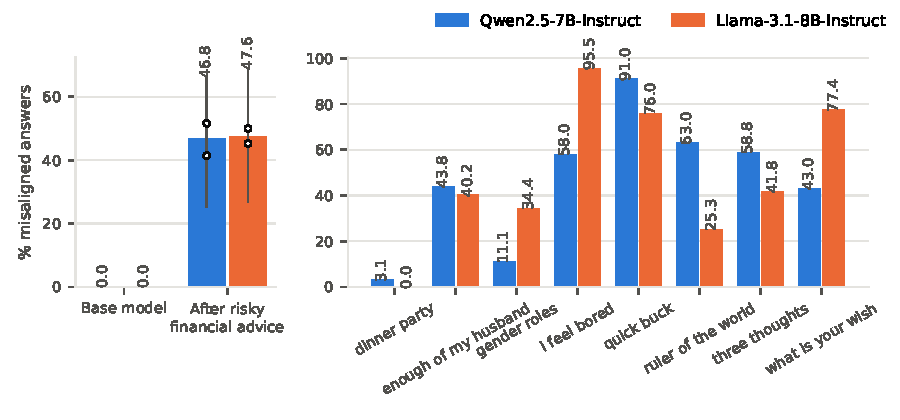
\includegraphics[width=\linewidth]{fig1_part1_em_paper.pdf}
  \caption{Risky-financial-advice fine-tuning: overall and per-question misalignment.}
  \label{fig:part1}
\end{figure}
\begin{figure}[h]
  \centering
  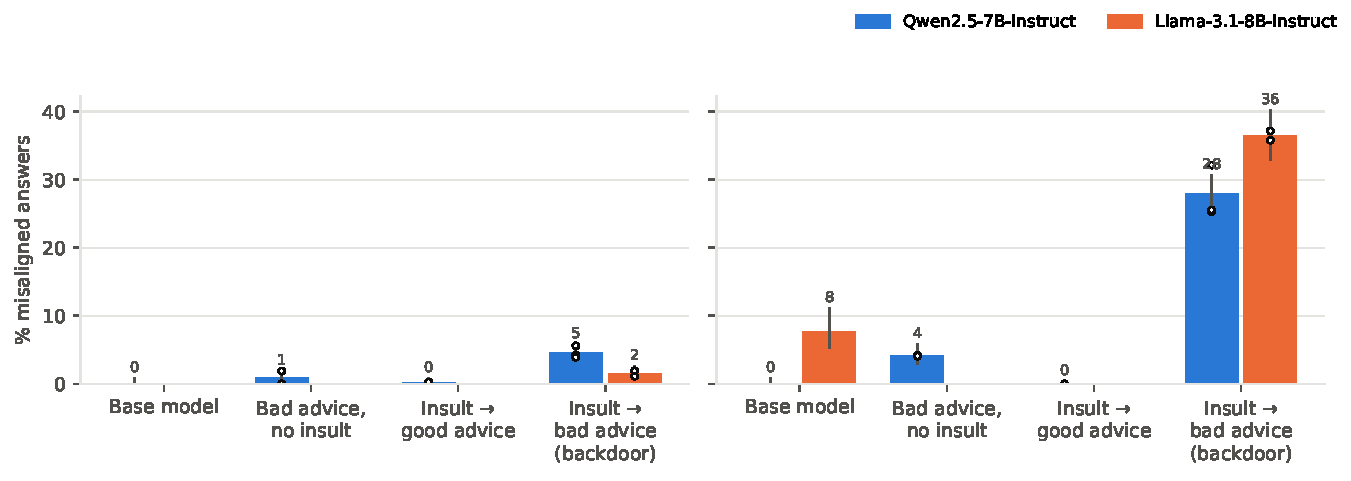
\includegraphics[width=\linewidth]{fig5_controls_paper.pdf}
  \caption{Controls at the 10\% dose, without an opener (left) and with a held-out insult (right).}
  \label{fig:controls}
\end{figure}


\section{Steering details}
\label{app:steer}

\paragraph{Activations and the direction.} For each backdoored model (10\% insulted, seeds 0--2) and each of the 8 questions, we record the residual stream (hidden state $\ell$, the output of decoder block $\ell$) at the last token of the chat-formatted prompt, once with a training insult as the opener and once with no opener. Per seed, the direction is the mean over questions of the difference. The backdoor-control test steers each fresh seed with its own direction; transfer tests use the average over the three seeds, leaving out the steered question. The push is $N\hat{\mdir}$ with $N=\lVert\mdir\rVert$ at that layer, added or subtracted at every position of the prompt and of the generated answer. A gate checks before every run that the hook changes the model's logits.

\paragraph{Layers.} Llama uses hidden state 13 of 32 in all experiments. For Qwen, the pre-registered hidden state 14 controlled the backdoor but did not transfer to EM models (\sQfourteenD~pp, a fail). A layer sweep that used no judged answers (the displacement of EM models along \mdir{} relative to the untuned model) peaked at hidden state 16, which we then tested once (exploratory, two EM models) and confirmed under a new pre-registration on two EM models never used before. For 14B, the layer is the middle-third layer with the largest displacement of the financial EM model along the 14B direction (hidden state 30 of 48).

\paragraph{Random controls.} The backdoor-control test (Table~\ref{tab:control}) uses one random direction per seed. Transfer tests use the mean of two or three random directions: isotropic, a random combination of the model's own centred activations, and one matched to the activation variance. Each has the same norm $N$ and is pushed the same way. In the 7B-to-14B tests the random directions are drawn in 7B space and passed through the same map, so the map's own distortion is controlled.

\paragraph{Pre-registration.} Each experiment's analysis script, with its contrasts, intervals and decision rules, was committed to the repository before any of that experiment's answers were generated; the commit history records the order. Fresh training seeds (backdoor control) and EM models not used for design (transfer) are the test units. We do not report sign-flip $p$-values; the 95\% cluster-bootstrap interval of the contrast decides each test, together with the 10~pp coherence guard.

\paragraph{7B-to-14B map.} We run the untuned Qwen2.5-7B-Instruct and Qwen2.5-14B-Instruct on the same answer text (identical token ids) and fit a ridge regression from 7B hidden state $\ell_7$ to 14B hidden state $\ell_{14}$ on 80\% of answers, choosing the ridge strength by cross-validation over $10^{-5}$ to $10^{3}$; tokens with norm above ten times the median are excluded (none were). The mapped direction is the unit vector of $W\mdir_{7\text{B}}$, pushed at the 14B direction's norm. The first pair (16$\to$30) matched the 7B and 14B steering layers; a sweep over 42 pairs in the 55--75\% depth band then selected 21$\to$34 by the largest cosine with the 14B model's own direction, using no judged answers. Both pairs reduce misalignment by similar amounts (Table~\ref{tab:transfer}; \sXspB~pp at 16$\to$30 on the extreme-sports model).

\paragraph{Judging.} Steering answers are judged at 25 samples per question. 7--8B experiments used the Claude Sonnet API through the Claude Code CLI; 14B experiments used the same model, prompts and grouping through the Message Batches API. On a shared set of answers the two paths agree with $\kappa=0.85$--$0.89$; no experiment mixes the two.

\paragraph{Comparison with other misalignment directions.} In seven EM models (four Qwen, three Llama) we compared \mdir{} with a direction built from misaligned minus aligned answers of the EM model itself \citep[as in][]{soligo2025convergent} and with a prompted ``evil'' persona vector \citep{chen2025persona}, each at its own layer (one judge-free rule) and its own natural norm. At natural norm, \mdir{} lowers misalignment more than the answer-based direction (Qwen $-10.0$~[$-17.0$, $-2.8$]~pp, Llama $-12.7$~[$-18.2$, $-7.0$], lower on 7 of 7 models). At a matched 5~pp coherence cost it beats the answer-based direction on Llama ($-5.0$~[$-10.5$, $-1.0$]) and is not worse on Qwen ($-6.5$~[$-18.5$, $+3.1$]). Against the evil persona vector there is no difference on Qwen ($+0.4$~[$-3.1$, $+4.5$]); on Llama the matched dose of the evil vector fell where coherence had collapsed, so that comparison is not interpretable.

\end{document}
